\documentclass[11pt]{article}

% Handle Spanish seamlessly!
\usepackage[utf8]{inputenc}
\usepackage[spanish, es-tabla]{babel}

% Change the language for the captions and default names
\renewcommand{\figurename}{Figura}

% Needed for the multline environment
\usepackage{amsmath}

% Images
\usepackage{graphicx}
\graphicspath{{Img/}}

\usepackage{geometry}
\geometry{
    a4paper,
    left = 20mm,
    right = 20mm,
    top = 15mm,
    bottom = 15mm
}

% Links please!
\usepackage{hyperref}

% Format the links
\hypersetup{
    pdfborder = {0 0 0},    % Remove the ugly border
    colorlinks = true,      % Let there be color
    citecolor = black,      % Make citations appear normal (i.e black)
    linkcolor = black,      % The same for links (i.e table of contents)
    urlcolor = cyan         % Color the web links. (cyan is fancy for blueish...)
}

\title{Configuración de \texttt{VPN}s en \texttt{capa 3}.}
\author{Pablo Collado Soto \\ \\ \textit{Ingeniería de Tráfico}}
\date{}

\begin{document}
    \maketitle

    \section{Introducción}
        En esta práctica configuramos $2$ \texttt{VPN}s de \texttt{capa 3} (\texttt{L3VPN}) con varias sedes. Para ello empleamos la tecnología \texttt{MPLS/LDP} para soportar los túneles así como \texttt{OSPF} para encaminar la red del proveedor y \texttt{BGP} para comunicar los \texttt{PE}s a través de los que podemos acceder a las distintas sedes. En definitiva, todo se reduce a configurar los diferentes encaminadores de manera correcta. Se pueden consultar las configuraciones de los encaminadores \href{https://github.com/UAH-s-Telematics-Engineering-Tasks/traff_eng/tree/master/P5/Router_confs}{aquí}.

    \section{Paso previo: conectividad \textit{Full-Mesh}}
        Antes de poner a funcionar la topología que se requiere empezamos por añadir una tercera sede a ambas \texttt{VPN}s. En este escenario intermedio cada \texttt{VPN} alcanza a las otras con un solo ``salto'' en el sentido de que se busca directamente el \texttt{PE} asociado a la \texttt{VPN} destino. Esto es, existe conectividad \textit{punto a punto} entre las \texttt{VPN}s. La forma de conseguir esto es forzar a cada \texttt{PE} a importar las rutas de todos los demás en base a los \texttt{RT}s (\textit{Routing Targets}) configurados. Todo se traduce a configurar el mismo \texttt{RT} para importar y exportar las rutas en cada \texttt{PE}. Eso sí, estos siguen siendo distintos para cada \texttt{VPN}. Las configuraciones se pueden consultar \href{https://github.com/UAH-s-Telematics-Engineering-Tasks/traff_eng/tree/master/P5/Router_confs/Full_mesh}{aquí}.

    \section{Topología final: \textit{Hub \& Spoke} y \textit{Star}}
        En la topología que se nos requería debemos configurar cada \texttt{VPN} de manera distinta. Es por eso que dedicamos una sección a cada una de ellas.

        \subsection{\texttt{VPN1}: \textit{Hub \& Spoke}}
            La topología \textit{Hub \& Spoke} se caracteriza por que todo el tráfico entre las sedes secundarias (\texttt{PE2} y \texttt{PE4}) pasa por la sede central (\texttt{PE1}). Para lograrlo veremos cómo se establecen en el fondo $2$ túneles distintos. Uno de ellos se encarga de comunicar a las sedes secundarias con la central mientras que el otro comunica ambas sedes secundarias \textbf{a través} de la central.\\

            La clave para lograr que esta estructura lógica funcione es forzar a las sedes secundarias (\textit{spokes}) a \textbf{solo} importar las rutas anunciadas por la sede central (\textit{hub}) mientras que la sede central importará las rutas anunciadas por ambas sedes secundarias. Podemos lograrlo tener este esquema a través de la configuración de los \texttt{RT}s de manera que la sede central exporta el \texttt{RT 101:222} e importa el \texttt{RT 103:222} mientras que cada \textit{spoke} importa el \texttt{RT 101:222} e importa el \texttt{RT 103:222}.\\

            El último detalle del que debemos encargarnos es de que el \textit{hub} exporte una ruta por defecto de manera que los \textit{spokes} encaminen tráfico a cualquier otra \texttt{VPN} a través de él. Así logramos que todo el tráfico de la \texttt{VPN1} tenga como primer destino la sede central si se origina en una sede secundaria y va destinado a la otra.

            Nos gustaría mencionar a modo de curiosidad que si no incluimos la linea \texttt{114} de la configuración de \href{https://github.com/UAH-s-Telematics-Engineering-Tasks/traff_eng/blob/master/P5/Router_confs/Hub_spoke_star/PE_1.cfg}{PE1} solo exportaremos la ruta por defecto a cada uno de los \textit{spokes} y no la ruta que nos lleva específicamente a la sede central desde cada sede secundaria. Esto se traduce en que en las tablas de encaminamiento de cada \textit{spoke} solo aparece la de la sede que tienen conectada y la ruta por defecto (\texttt{0.0.0.0}). Así, todo paquete que que sea emitido por una sede secundaria, ya vaya a la otra sede secundaria o a la central, llevará la misma etiqueta a nivel de \texttt{VPN}. Ya que el ejemplo que se ofrece en el guión de la práctica contiene la línea en cuestión veremos que en el fondo, y tal y como adelantábamos al inicio de la sección, en el fondo tenemos ``2'' túneles desde cada \textit{spoke}, cada uno con su correspondiente etiqueta. Uno de ellos irá a la sede central y otro a la otra sede secundaria \textbf{a través} de la sede central.\\

        \subsection{\texttt{VPN2}: \textit{Star}}
            En este caso la estructura lógica es idéntica a la anterior salvo por un pequeño detalle: debemos eliminar la conectividad entre las sedes secundarias. Dado que para esta \texttt{VPN} la sede central es \texttt{PE2} en vez de \texttt{PE1} solo debemos evitar que \texttt{PE2} publique una ruta por defecto como lo estaba haciendo \texttt{PE1} en la topología anterior. Esto implica que la configuración de la topología \textit{star} es ``más sencilla'' en cuanto a que requiere un paso de configuración menos. Al igual que antes, ahora \texttt{PE2} debe importar los \texttt{RT}s de ambas sedes secundarias (\texttt{RT 104:222}) (\texttt{PE1} y \texttt{PE4}) y exportar el suyo propio (\texttt{RT 102:222}). Tanto \texttt{PE1} como \texttt{PE4} importaran \textbf{solo} el \texttt{RT} de \texttt{PE2} mientras que exportarán el mismo.\\

            Con lo anterior se elimina la conectividad entre sedes secundarias tal y como se requiere.\\

        \subsection{Índice de figuras con las comprobaciones}
            Ya que vamos a incluir $17$ figuras hemos recopilado en una pequeña lista las que se refieren a cada nodo de la red. Nótese que los números de la lista están enlazados a las propias figuras.

            \begin{itemize}
                \item \texttt{PE1}:
                    \begin{itemize}
                        \item \texttt{Genéricas}: \ref{fig:ip_route_PE_1}, \ref{fig:mpls_table_PE_1}, \ref{fig:trace_10.1.1.2_PE_1}.
                        \item \texttt{VPN1}: \ref{fig:ip_bgp_VPN1_PE_1}, \ref{fig:trace_10.10.2.1_PE_1}, \ref{fig:trace_10.10.3.1_PE_1}.
                        \item \texttt{VPN2}: \ref{fig:ip_bgp_VPN2_PE_1}.
                    \end{itemize}
                \item \texttt{PE2}:
                    \begin{itemize}
                        \item \texttt{Genéricas}: \ref{fig:mpls_table_PE_2}.
                        \item \texttt{VPN1}: \ref{fig:ip_bgp_VPN1_PE_2}, \ref{fig:trace_10.10.1.1_PE_2}, \ref{fig:trace_10.10.3.1_PE_2}.
                        \item \texttt{VPN2}: \ref{fig:ip_bgp_VPN2_PE_2}, \ref{fig:trace_10.20.1.1_PE_2}, \ref{fig:trace_10.20.3.1_PE_2}.
                    \end{itemize}
                \item \texttt{PE4}:
                    \begin{itemize}
                        \item \texttt{VPN1}: \ref{fig:ip_bgp_VPN1_PE_4}.
                        \item \texttt{VPN2}: \ref{fig:ip_bgp_VPN2_PE_4}.
                    \end{itemize}
                \item \texttt{P3}:
                    \begin{itemize}
                        \item \texttt{Genéricas}: \ref{fig:mpls_table_P_3}.
                    \end{itemize}
            \end{itemize}

        % PE1 Figures
            \begin{figure}
                \centering
                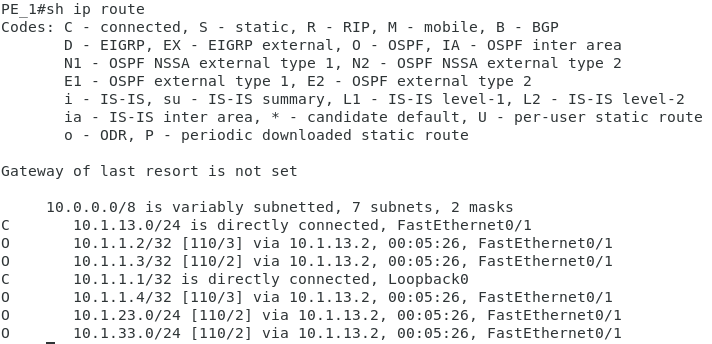
\includegraphics[width=0.6\linewidth]{ip_route_PE_1.png}
                \caption{Tabla de encaminamiento genérica de \texttt{PE1}}
                \label{fig:ip_route_PE_1}
            \end{figure}

            \begin{figure}
                \centering
                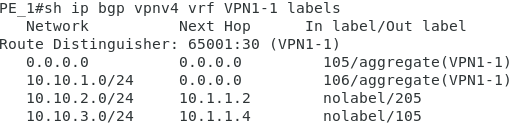
\includegraphics[width=0.6\linewidth]{ip_bgp_VPN1_PE_1.png}
                \caption{Tabla de encaminamiento \texttt{BGP} de la \texttt{VPN1} de \texttt{PE1}}
                \label{fig:ip_bgp_VPN1_PE_1}
            \end{figure}

            \begin{figure}
                \centering
                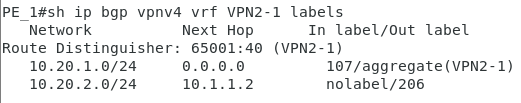
\includegraphics[width=0.6\linewidth]{ip_bgp_VPN2_PE_1.png}
                \caption{Tabla de encaminamiento \texttt{BGP} de la \texttt{VPN2} de \texttt{PE1}}
                \label{fig:ip_bgp_VPN2_PE_1}
            \end{figure}

            \begin{figure}
                \centering
                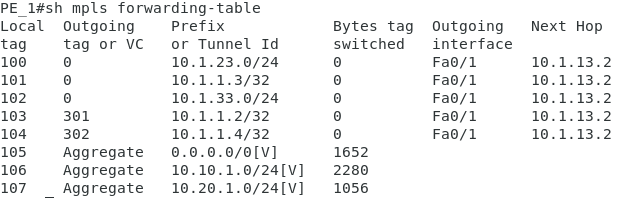
\includegraphics[width=0.6\linewidth]{mpls_table_PE_1.png}
                \caption{\texttt{LFIB} de \texttt{PE1}}
                \label{fig:mpls_table_PE_1}
            \end{figure}

            \begin{figure}
                \centering
                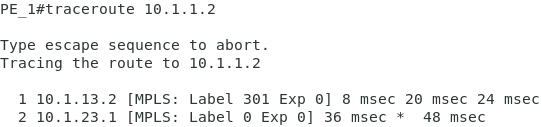
\includegraphics[width=0.6\linewidth]{trace_10.1.1.2_PE_1.png}
                \caption{\texttt{Traceroute} a \texttt{10.1.1.2} desde \texttt{PE1}}
                \label{fig:trace_10.1.1.2_PE_1}
            \end{figure}

            \begin{figure}
                \centering
                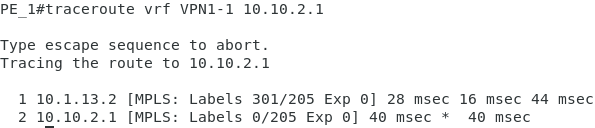
\includegraphics[width=0.6\linewidth]{trace_10.10.2.1_PE_1.png}
                \caption{\texttt{Traceroute} a \texttt{10.10.2.1} (\texttt{VPN1}) desde \texttt{PE1}}
                \label{fig:trace_10.10.2.1_PE_1}
            \end{figure}

            \begin{figure}
                \centering
                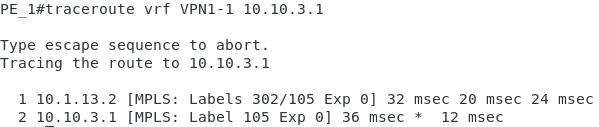
\includegraphics[width=0.6\linewidth]{trace_10.10.3.1_PE_1.png}
                \caption{\texttt{Traceroute} a \texttt{10.10.3.1} (\texttt{VPN1}) desde \texttt{PE1}}
                \label{fig:trace_10.10.3.1_PE_1}
            \end{figure}

        % PE2 Figures
            \begin{figure}
                \centering
                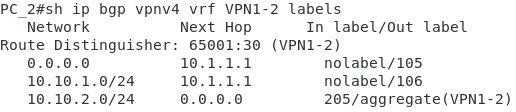
\includegraphics[width=0.6\linewidth]{ip_bgp_VPN1_PE_2.png}
                \caption{Tabla de encaminamiento \texttt{BGP} de la \texttt{VPN1} de \texttt{PE2}}
                \label{fig:ip_bgp_VPN1_PE_2}
            \end{figure}

            \begin{figure}
                \centering
                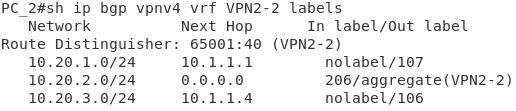
\includegraphics[width=0.6\linewidth]{ip_bgp_VPN2_PE_2.png}
                \caption{Tabla de encaminamiento \texttt{BGP} de la \texttt{VPN2} de \texttt{PE2}}
                \label{fig:ip_bgp_VPN2_PE_2}
            \end{figure}

            \begin{figure}
                \centering
                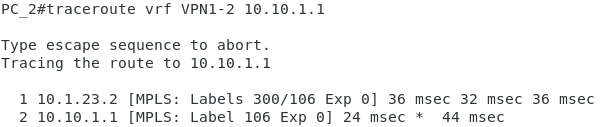
\includegraphics[width=0.6\linewidth]{trace_10.10.1.1_PE_2.png}
                \caption{\texttt{Traceroute} a \texttt{10.10.1.1} (\texttt{VPN1}) desde \texttt{PE2}}
                \label{fig:trace_10.10.1.1_PE_2}
            \end{figure}

            \begin{figure}
                \centering
                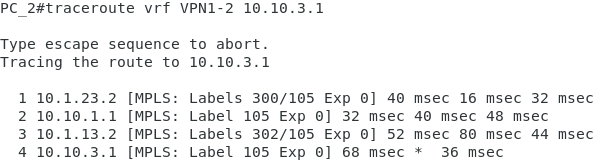
\includegraphics[width=0.6\linewidth]{trace_10.10.3.1_PE_2.png}
                \caption{\texttt{Traceroute} a \texttt{10.10.3.1} (\texttt{VPN1}) desde \texttt{PE2}}
                \label{fig:trace_10.10.3.1_PE_2}
            \end{figure}

            \begin{figure}
                \centering
                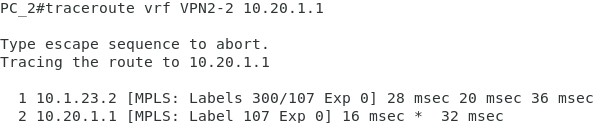
\includegraphics[width=0.6\linewidth]{trace_10.20.1.1_PE_2.png}
                \caption{\texttt{Traceroute} a \texttt{10.20.1.1} (\texttt{VPN2}) desde \texttt{PE2}}
                \label{fig:trace_10.20.1.1_PE_2}
            \end{figure}

            \begin{figure}
                \centering
                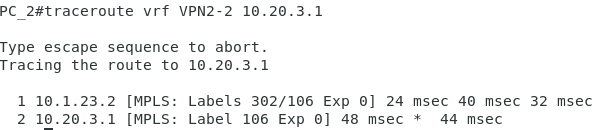
\includegraphics[width=0.6\linewidth]{trace_10.20.3.1_PE_2.png}
                \caption{\texttt{Traceroute} a \texttt{10.20.3.1} (\texttt{VPN2}) desde \texttt{PE2}}
                \label{fig:trace_10.20.3.1_PE_2}
            \end{figure}

            \begin{figure}
                \centering
                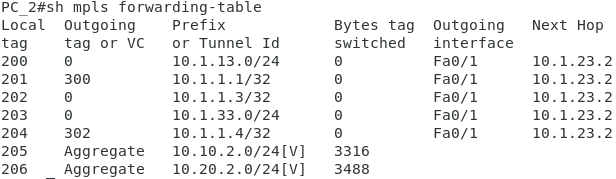
\includegraphics[width=0.6\linewidth]{mpls_table_PE_2.png}
                \caption{\texttt{LFIB} de \texttt{PE2}}
                \label{fig:mpls_table_PE_2}
            \end{figure}

        % PE4 Figures
            \begin{figure}
                \centering
                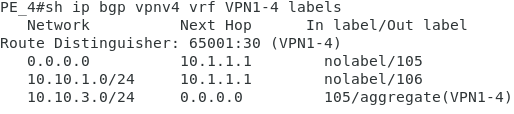
\includegraphics[width=0.6\linewidth]{ip_bgp_VPN1_PE_4.png}
                \caption{Tabla de encaminamiento \texttt{BGP} de la \texttt{VPN1} de \texttt{PE4}}
                \label{fig:ip_bgp_VPN1_PE_4}
            \end{figure}

            \begin{figure}
                \centering
                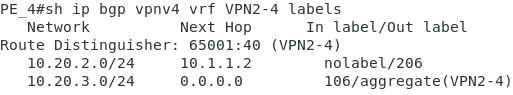
\includegraphics[width=0.6\linewidth]{ip_bgp_VPN2_PE_4.png}
                \caption{Tabla de encaminamiento \texttt{BGP} de la \texttt{VPN2} de \texttt{PE4}}
                \label{fig:ip_bgp_VPN2_PE_4}
            \end{figure}

        % P3 Figures
            \begin{figure}
                \centering
                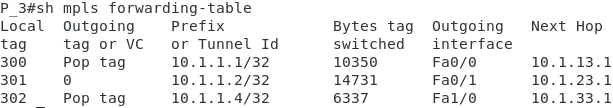
\includegraphics[width=0.6\linewidth]{mpls_table_P_3.png}
                \caption{\texttt{LFIB} de \texttt{P3}}
                \label{fig:mpls_table_P_3}
            \end{figure}

    \section{Conclusiones}
            Tras realizar la práctica vemos cómo la configuración de \texttt{VPN}s a nivel de red es tremendamente versátil y que cambios rápidos y escuetos nos permiten alterar tremendamente la topología.
\end{document}
